\subsection{EMT-Linux with x86-64 MMU Drivers}
\label{emt:sec:impl}

\noindent
We develop EMT on Linux, referred to as EMT-Linux.
Conceptually, it took four steps:
1) identifying memory management code in architecture-independent modules 
    that are hardwired to x86-like, tree-based translation scheme;
2) rewriting them using the EMT API;
3) moving architecture-specific optimizations 
    into
%    (e.g., ``\texttt{\small arch/x86/mm}'')
	the x86-64 MMU driver,
and 4) writing default implementations of 
    customizable functions.

% git diff --stat 4a17158dfa32c348bb4af8d8a24fdadc9bb69fb8 HEAD -- arch/x86 | grep enhanced
% git diff --stat 4a17158dfa32c348bb4af8d8a24fdadc9bb69fb8 arch/x86/include/asm/pgtable.h
%  2005  git diff --stat 4a17158dfa32c348bb4af8d8a24fdadc9bb69fb8 HEAD -- mm/*
%  2007  git diff --stat 4a17158dfa32c348bb4af8d8a24fdadc9bb69fb8 HEAD -- arch/x86 | grep enhanced
%  2008  git diff --stat 4a17158dfa32c348bb4af8d8a24fdadc9bb69fb8 HEAD -- include/

The EMT implementation on Linux (v5.15)
    takes 9.5K lines of code changes 
	(7.3K for interface refactoring and 2.2K for the x86-64 MMU driver)
    in 15 person-months.
%  (including testing and profiling).
We changed 196 kernel functions in the \texttt{\small mm} directory of Linux---most 
    memory management code interacts with the page table.
%    (the only exceptions are \REVIEW{memory allocators} and \REVIEW{VMA management}).

We use macros and inline functions
	to minimize interface overhead as per Linux's coding style~\cite{linux:code:icache}; 
	\texttt{\small \#ifndef}-based function redirections are used otherwise.
Specifically, we turn functions no more than three lines into macro or inline functions. 
% we use macros only to decide the right functions 
% 	to call, instead of turning big code into macros.
We ensure that EMT does not break performance characteristics, e.g., 
	no increase of stack size or call stacks, and no decrease 
	of instruction cache hit rates in most cases (\S\ref{emt:sec:eval:eval-EMT-radix-vs-vanilla}). 
% The measured instruction cache hit rates
% 	of EMT-Linux is almost the same as vanilla Linux.
% \schai{The measured instruction cache hit rates on EMT-Linux differ from those on vanilla Linux by at most 0.8\%}.
%	cache hit rates (\S\ref{emt:sec:eval:eval-EMT-radix-vs-vanilla}).

%	which are replaced by architecture-specific
%    code at compile time.
% \TODO{TODO: there is a big discussion on low-overhead runtime checks in the discussion
%	and we shall briefly talk about them here.}

%We transformed architecture-specific Linux
 %   routines into architecture-neutral EMT APIs;
Moreover, we preserve {\it all} of Linux's existing architecture-specific optimizations
	%    that manipulate the radix-tree page table
	and realize them in the x86-64 MMU driver.
Hence, EMT supports all virtual memory features of vanilla Linux and
	is {\it transparent} to user applications.

% Refactored code under \texttt{/mm} forlder 
% with \interface takes about 6.5k LOC.
% \JZc{Shall we also mention person-month used?}. 
% \schaic{person-month is a bit hard to estimate, since we developing the interface during the research process.}
% \schai{The refactoring of the common code base takes roughly 12-14 months single person}.
% We add a new header file, \texttt{include/linux/pgtable\_enhanced.h} that
% defines all functions of \interface. \mmudrivers are implemented under an
% architecture-specific directory. For example, x86's Radix driver is implemented in 
% \texttt{arch/x86/mm/pgtable\_enhanced.c} and ECPT driver is in
% \texttt{arch/x86/mm/ecpt.c}.


% \jyk{We can provide anexample.} 
% \schaic{I don't know if we want to reinforce that much about macro redirection.
% It has a drawback 
% of making the code fixed at compile time. If we make some argument that 
% translation architecture can be changed at runtime, this could be a problem.}
% \schai{Our evaluation (\S\ref{emt:sec:eval:eval-EMT-radix-vs-vanilla}) show that EMT has negligible overhead (within the standard deviation)}.
% of application performance overhead.
% in section \ref*{sec:eval:eval-EMT-radix-vs-vanilla}} 

% In implementing the interface and refactoring the x86 codebase based on it, we
% focus on minimizing the performance impact of the implementation. To this end,
% we make extensive use of macros to implement the functions defined in the
% \interface specification. Hence, we try to connect the prototypes defined in the
% \interface directly to the corresponding x86 implementation at compile time via
% macros. We have found that this approach is feasible and effective. Our
% evaluation demonstrated that it caused less than 0.1\% performance overhead and
% did not cause any hindrance in switching to ECPT.

% \paragraph{Function pointer structure.} \jyk{This paragraph may be removed if
% there is not much thing to mention. Function pointer is used for 1)
% registering architecture-specific functions, 2) registering memory translation
% scheme (\hwofg).} Architecture-specific optimization functions are registered to
% \interface as function pointers. \jyk{Give an example source code.} \jyk{No
% overhead introduced.} \jz{\optgrps all have default implementation provided, and
% the re-implementation of \optgrps should not affect the correctness of the
% system.}

\begin{figure}[H]
	\centering
\begin{minted}[xleftmargin=17.5pt,linenos,mathescape,breaklines,fontsize=\scriptsize,escapeinside=@@]{C}
void walk_tobj_range(start, end, walk) {
  struct tlock lock; struct tobj_iter iter;
  struct tobj tobj; ulong size; 
  struct tdb *tdb = walk->mm->tdb;
  err = @\codehl{emtlock}{addr\_range\_get\_lock}{}@(tdb, start, end, &lock);
  addr_range_write_lock(&lock);
  err = tobj_iter_init(tdb, start, end, &iter);
  ...
  while (tobj_iter_has_next(iter)) {
    err = @\codehl{emtiter}{tobj\_iter\_next}@(&iter, &tobj);
    err = tobj_read_attr(&tobj, TOBJ_ATTR_SIZE, &size);
    err = walk->ops->@\codehl{emtptr}{tobj}@(tobj, tobj->va, tobj->va + size, walk);
    ...
  }
  tobj_iter_end(&iter);
  addr_range_write_unlock(&lock);
  addr_range_put_lock(&lock);
} /* mm/pagewalk.c */
\end{minted}

\caption{\bf Rewriting code in Figure~\ref{emt:fig:need:linux-performance-opt} with EMT.}
\label{emt:fig:interface-compare}
%\vspace{-5pt}
\end{figure}

% no space for them
\begin{comment}
\begin{figure}[H]
	\centering
	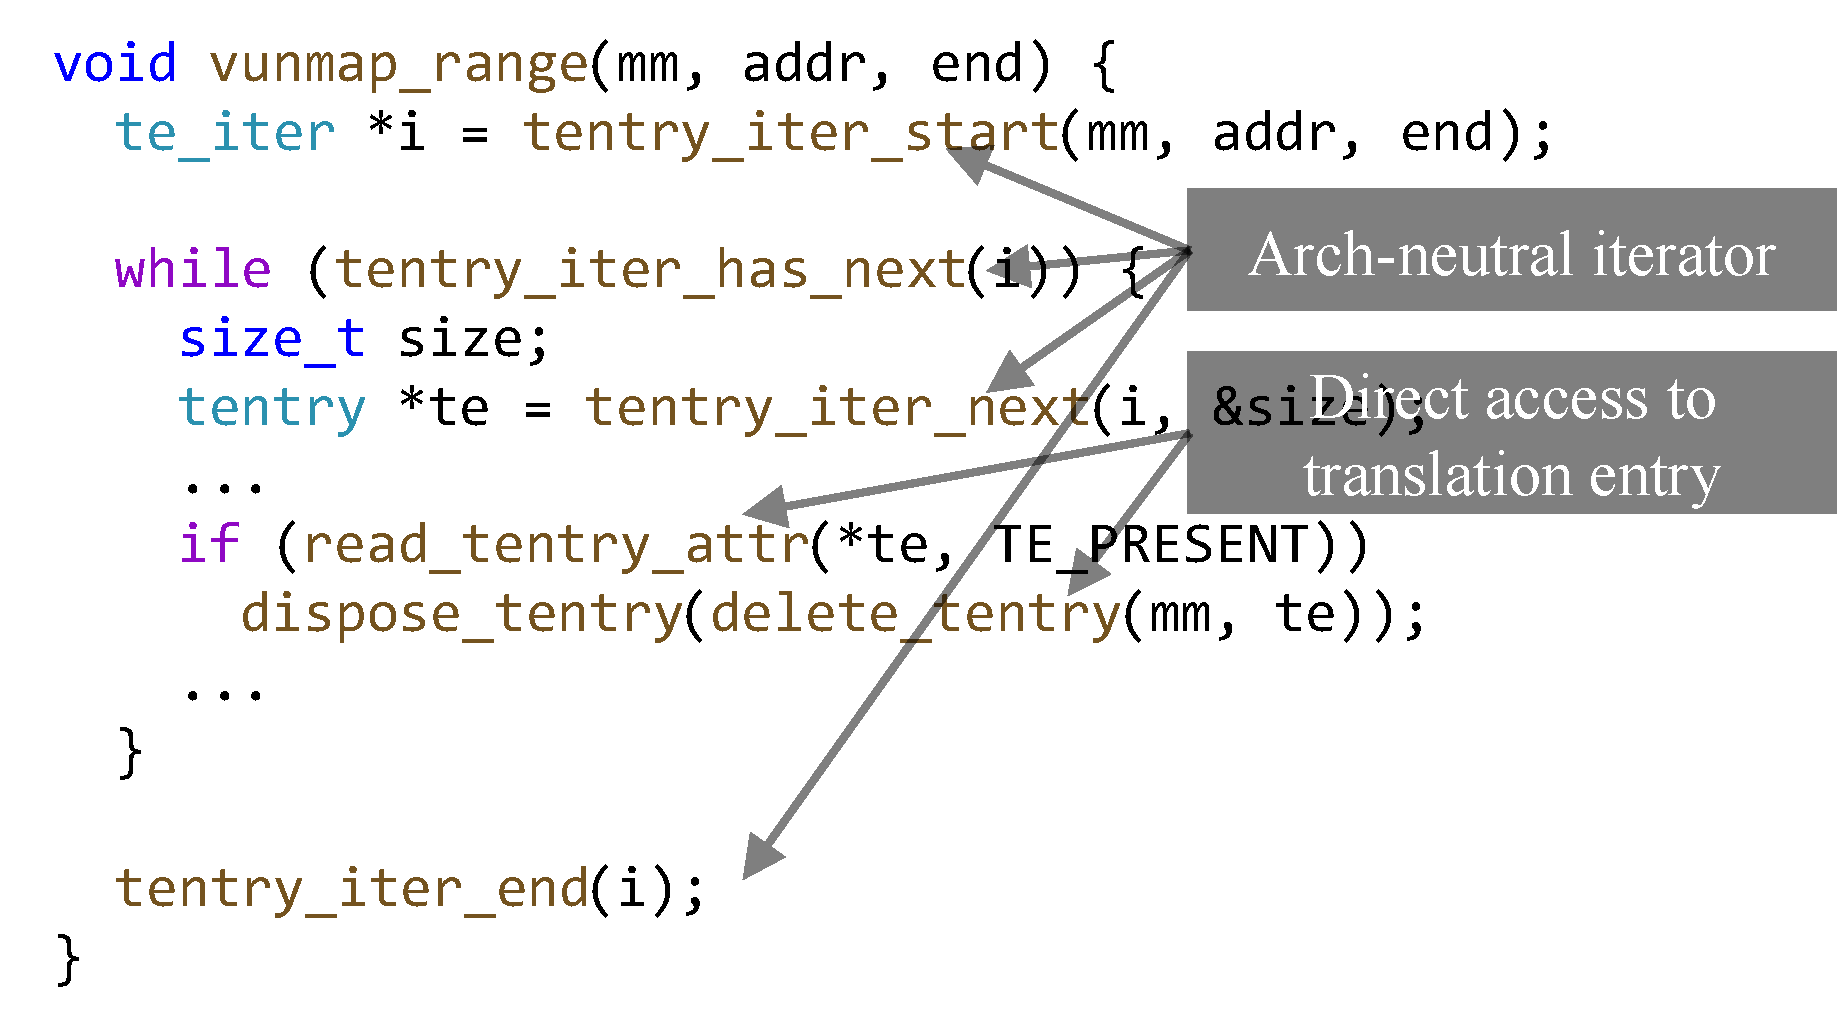
\includegraphics[width=0.5\textwidth]{figs/linux-no-interface-new}
	\caption{\bf An example of Linux's memory management code refactored with no tree assumption. \TODO{Improve fig}}
	\label{emt:fig:impl:refactor}
\end{figure}

\begin{figure}[H]
	\centering
	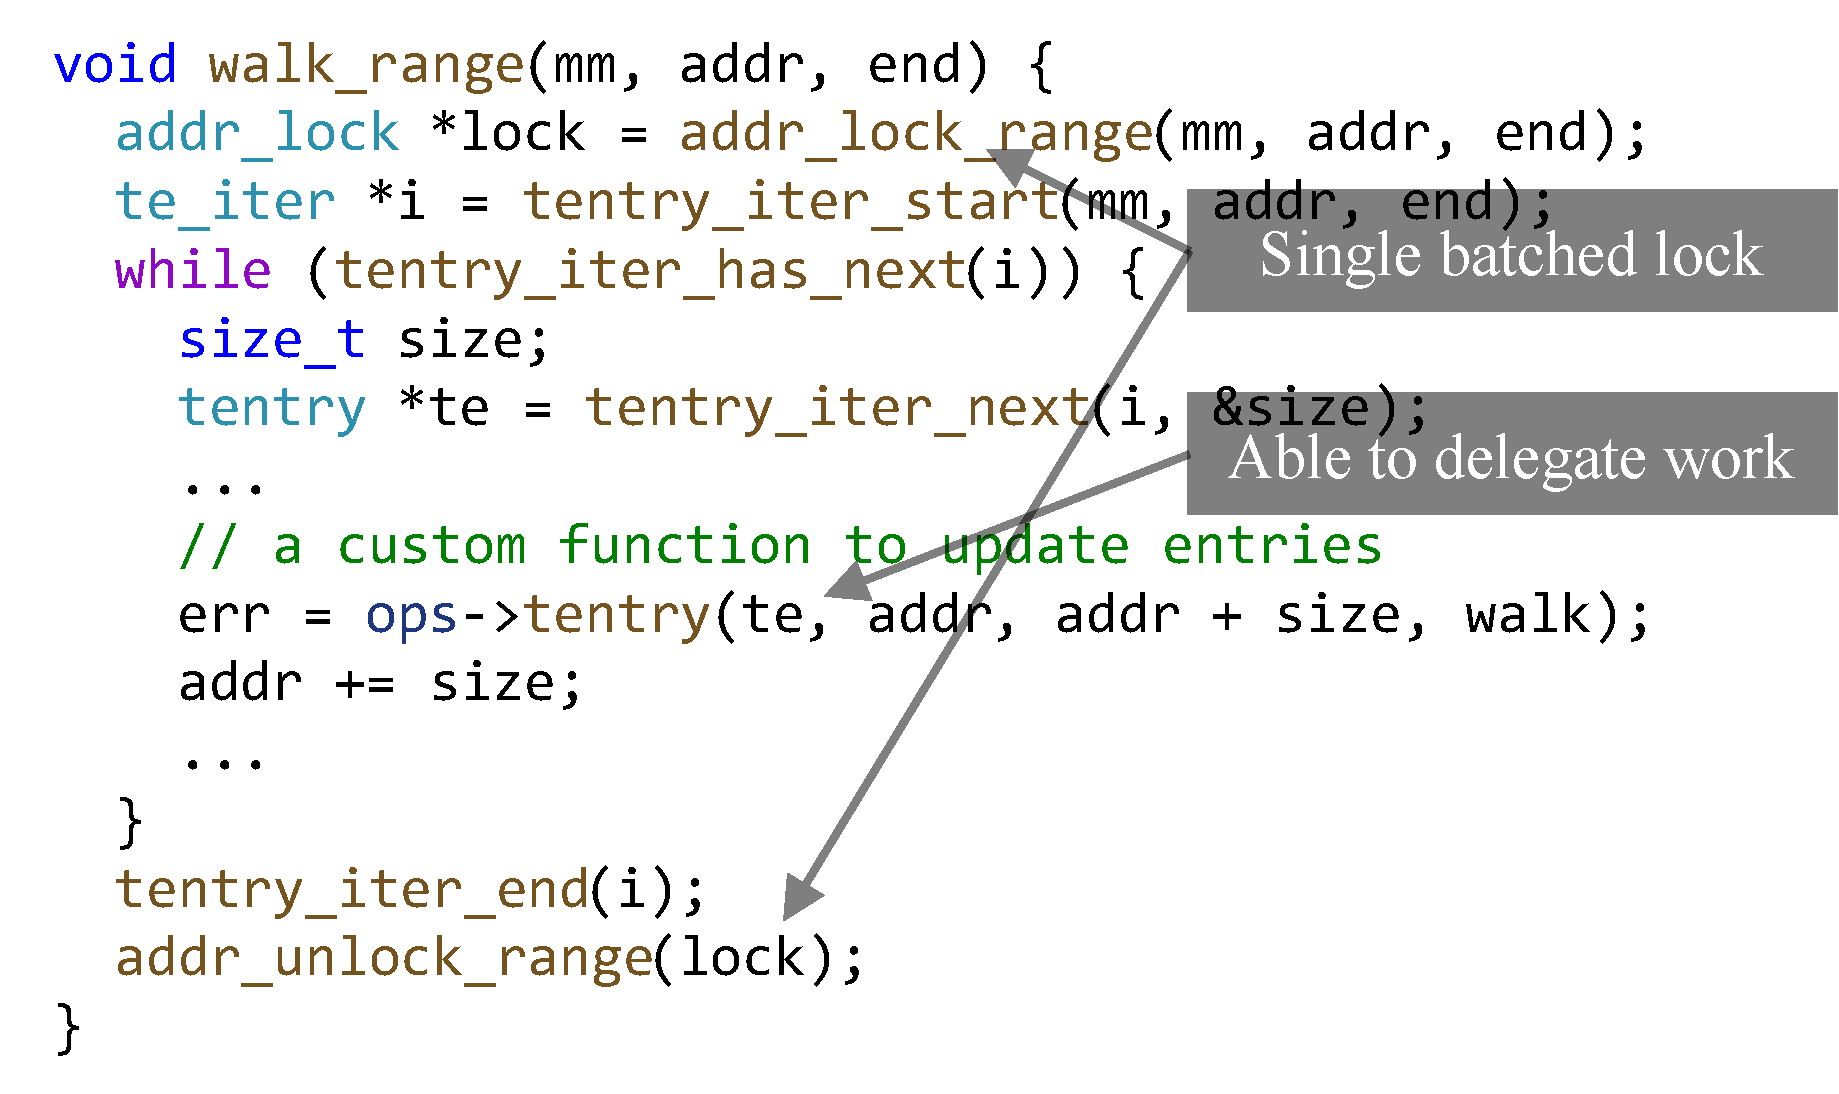
\includegraphics[width=0.5\textwidth]{figs/linux-performance-opti-new}
	\caption{\bf Low-level optimizations in Linux code kept after refactoring. \TODO{TODO}}
	\label{emt:fig:need:linux-performance-opt-new}
\end{figure}
\end{comment}

% Linux already has well-defined routines
%    for manipulating page tables and entries,
%	despite being 
%   specific to tree-based translation.

% A few tricky cases come from kernel routines with overloaded semantics 
% % which only make sense with the radix tree structure 
%	(e.g., Figure~\ref{emt:fig:need:linux-no-interface});
%    we did not understand certain semantics which 
%    caused issues on ECPT (\S\ref{emt:sec:ecpt_impl}).
% This again shows the importance of a well-defined OS interface.

% Refactoring Linux code with the EMT customizable functions is more challenging,
%    because performance is harder to understand statically. % in a static way.
% With vanilla Linux as a reference,

% fine-grained locks
%    by locking a page-table page ()
%   using the PMD entry.

%    intermediate translation entries (e.g., a L2 page table entry).

% Figures~\ref{emt:fig:impl:refactor} and~\ref{emt:fig:impl:refactor} shows the refactored code of 
 %   the vanilla Linux code in Figure~\ref{emt:fig:need:linux-no-interface} 
 %   and~\ref{emt:fig:need:linux-performance-opt}, respectively.

% In general, there are two ways to redirect the interface functions 
%	its MMU driver implementation: 
%	1) Use config macro to control which function will be called at compile time;
%	2) Define a set of function pointers which can be registered at init run time.
% We follow Linux's convention to connect the interface functions with
%	appropriate function calls using config macros.
% This reduce the overhead of function calls by increasing the chance of inlining.
%\schai{We demonstrate that it causes less than 0.5\% of application performance overhead.
% in section \ref*{sec:eval:eval-EMT-radix-vs-vanilla}} 
% \schaic{The code example here is mainly to help udnerstanding;
%	I don't think this would be super neccessary in the final paper
%	as this is more or less following Linux's convention.}

\begin{comment}
\begin{figure}[H]
	\centering
% Adapted from https://github.com/freebsd/freebsd-src/blob/main/sys/compat/linuxkpi/common/src/linux_page.c#L246
\begin{minted}[xleftmargin=20pt,tabsize=4,linenos,mathescape,breaklines,fontsize=\footnotesize]{C}

// declaration in EMT interface
pte_t * pte_iter_next(i);

// code usage
while (pte_iter_has_next(i)) {
	// arch-defined iteration progression
	pte_t *ptep = pte_iter_next(i);
	... // do something
}


#define ARCH_HAS_PTE_ITER_NEXT
// radix specific implementation
// arch/x86/mm/radix.h
static inline pte_t * pte_iter_next(i) {
	if (at_boundary(i)) {
		return locate_pte(i->mm, i->addr + i->pg_size, 
			i->pg_size, NULL /* no hint */);
	}
	return ++(i->pte);
}

// generic implementation
// include/linux/EMT-default.h
#ifndef ARCH_HAS_PTE_ITER_NEXT
static inline pte_t * pte_iter_next(i) {
	return locate_pte(i->mm, i->addr + i->pg_size, 
		i->pg_size, NULL /* no hint */);
}
#endif
\end{minted}

\caption{Simplified code for Macro redirection}
\label{emt:code:PFhandler}
\end{figure}

\subsubsection{Refactoring \essgrps}
\schaic{What's easy?}
Refactoring it with \essgrps is a relative straightforward process.
The reason is that Linux already provides routines to 
insert, update, locate,
	and delete entries from translation structure 
	(radix page table in Linux's conception).
\schaic{Before this part, reader should already know that these functions in linux are not working.
Let me know if you think this won't be clear}
For example, \texttt{set\_pte\_at(mm, addr, ptep, pte)} 
	inserts a new PTE with value \texttt{pte} at the address \texttt{addr} in the page table \texttt{mm};
\texttt{pmd\_offset(pud, addr)} 
	locates a pmd pointer in the page table at the address \texttt{addr} with auxiliary upper level page table entry \texttt{pud}.
They are conducting the job of translation structure manipulation 
	but just with over-simplified interface for a five-level tree structure.
We locate the functions and replace it with our enhanced interface 
	by supplementing the missing information like page table root, page size.

Similar things happen for translation entry operations but with more engineering efforts
	due to the huge number of functions in this group.
Linux comes with 121 functions to read and write pte entries attributes.
We didn't develop new attributes of PTEs, but \branding provides the chance
	for future kernel developers to add new attributes they want from PTEs.
We locate the functions and replace it with our translation entry interface.
For example, \texttt{pte\_present(pte)} checks if the mapping represented by PTE is present;
	it is replaced with \texttt{read\_pte\_attr(pte, PTE\_PRESENT)} in \branding.
In our deployment of \interface, we use macro to redirect the function calls to 
	MMU driver to reduce function call overhead;
For example, in radix, \texttt{read\_pte\_attr(pte, PTE\_PRESENT)} will be redirected to 
\texttt{radix\_native\_pte\_present(pte)}.
Besides performance benefit, macro redirection can force developers to detect 
	missing implemenation at compile time.
It triggers a compilation error, much desirable than a runtime error,
	if the function is not implemented in the MMU driver.

\subsubsection{Refactoring \optgrps}
\para{Nonlinearity of interface development} \schaic{What's hard?}
While refactoring with \essgrps is relative straightforward, 
	refactoring with \optgrps is a more complicated process.
The design of new interface is not a linear process,
	one may not be able to design an interface with complete semantics and correct performance implications
until testing the implementation of driver.

\begin{figure}[H]
	\centering

% Adapted from https://github.com/freebsd/freebsd-src/blob/main/sys/compat/linuxkpi/common/src/linux_page.c#L246

\begin{minted}[xleftmargin=20pt,linenos,mathescape,breaklines,fontsize=\footnotesize]{C}
// 1 walk for Radix, ECPT unsupported
// walking higher level page table entries
...
pmd_t *pmd = pmd_offset(pud, addr);
// Assumes page table structure
if (pmd_none(pmd) && __thp_enabled(vma)) {
	// try to create huge page mapping
	return create_huge_pmd(vma, addr, pmd, ...);
}

// handle specific 4KB fault
handle_pte_fault(vma, pmd, addr);


int aspace_void(mm, addr, upper_gran_hint, pg_size)
{
	return !pte_is_huge(mm, addr, upper_gran_hint, pg_size) 
		&& !pte_is_directory(mm, addr, upper_gran_hint, pg_size)
	 	&& !pte_is_partial_built(mm, addr, upper_gran_hint, pg_size);
}

// refactored with EMT aspace_void
pmd_t *pmd = locate_pte(mm, pud, addr);
// Assumes page table structure
if (aspace_void(mm, addr, pmd, PMD_SIZE) && __thp_enabled(vma)) {
	// try to create huge page mapping
	return create_huge_pmd(vma, addr, pmd, ...);
}

// handle specific 4KB fault
handle_pte_fault(vma, pmd, addr);

\end{minted}

\caption{Simplified code for Linux PF handler}
\label{emt:code:PFhandler}
\end{figure}

For example, while we are working with the PF handler (Figure~\ref{emt:code:PFhandler}) in linux kernel,
	we realize that the \texttt{pmd\_none} function 
	conveys a overloading semantics that is neither a huge page or a directory mapping.
Thus, we tried to replace it with \texttt{pte\_is\_huge} and \texttt{pte\_is\_directory}.
The two meanings are enough in radix context since the pmd entry can only be one of them.
However, for architecture that all page table entries are data page entries, like ECPT, it will never be directory mapping.
Thus, we must introduce a third meaning to \texttt{pte\_is\_partial\_built}
	to check if the address space has \textit{any} mapping inside the range.
Otherwise, if kernel doesn't know the information and only relies on huge and directory checks,
	it may build a a huge page mapping while there are 4KB page mappings inside the range.
In such way,
	it will lead to duplicated mappings for same VA range,
	an irresolvable behavior for hardwares,
	and potential lost of data.

Until so far, after deeply understand the Linux's PF handler code,
	we develop the \texttt{aspace\_void} function to check if the address space's mapping properties.
It achieves the same function while preserving radix's great optimization
	of using the pmd entry's semantic in tree structure.
This seems to be a good balance until ECPT's MMU driver is implemented.
For ECPT, its \texttt{pte\_is\_partial\_built} implementation may contain a loop
	to check all page table entries inside the range
	since its high granularity page table entries contain no info about low granularity entries.
This could expose a performance issue since \texttt{\_\_thp\_enabled(vma)} 
	can be either the cheaper check (ECPT) or more expensive check (Radix)
	depends on the MMU driver implementation.
For Radix, one may prefer to have the \texttt{aspace\_void} check first
	and then the \texttt{\_\_thp\_enabled(vma)} check
	since the former one only checks one property.
\schaic{This can be confirmed with our later profiling: 
	\texttt{\_\_thp\_enabled(vma)} is 2x more expensive check than \texttt{aspace\_void} check
	in radix with THP enabled}
However, for ECPT, we want to have the \texttt{\_\_thp\_enabled(vma)} check goes first
	since it can help filter out many cases before the expensive \texttt{aspace\_void} check.
An extreme of such effect's optimization is when THP is disabled,
	\texttt{\_\_thp\_enabled(vma)} will return false and the \texttt{aspace\_void} check will be skipped.
It won't be possible to handle both case without modifying PF handler's
	arch-neutral code.

\begin{figure}[H]
	\centering

% Adapted from https://github.com/freebsd/freebsd-src/blob/main/sys/compat/linuxkpi/common/src/linux_page.c#L246

\begin{minted}[xleftmargin=20pt,linenos,mathescape,breaklines,fontsize=\footnotesize]{C}

// default implementation
static inline int aspace_placement(mm, addr, vma ...)
{
	return __thp_enabled(vma) && aspace_void(mm, addr ...);
}

// ECPT implementation
static inline int aspace_placement(mm, addr, vma ...)
{
	return aspace_void(mm, addr ...) && __thp_enabled(vma);
}


// refactored with EMT aspace_placement
pmd_t *pmd = locate_pte(mm, pud, addr);
// Assumes page table structure
if (aspace_placement(mm, addr, vma ...)) {
	// try to create huge page mapping
	return create_huge_pmd(vma, addr, pmd, ...);
}

// handle specific 4KB fault
handle_pte_fault(vma, pmd, addr);

\end{minted}

\caption{Simplified code for Linux PF handler}
\label{emt:code:PFhandler}
\end{figure}

Based on this observation, thanks to the extensibility of \optgrps functions,
	we introduce a new optimization function \texttt{aspace\_placement} (\schaic{I need a better name than this})
	to direct the order of the two checks.
For Radix, it can just inherit the default implementation
	which has the \texttt{aspace\_void} check first.
For ECPT, it can override the default implementation, 
	with whatever order it favors.
In a longer vision, we may wish to provide a more generic performance interface
	that allow developers to define the order of the checks.

We know that such optimizations can happen in many places in the kernel,
	and what we spotted here is only a tip of the iceberg.
	\branding welcomes the future developers to add more optimization functions
	that can bring more performance beneifts while not losing extensibility.


\para{Range operation refactoring}
A common routine in linux kernel is to operate on a range of virtual addresses.
In fact, in our refactoring experience,
	besides PF handler and GUP (Get User Pages) routine,
	range operations are the most common place where we need to refactor.
We spotted 40 places in \texttt{/mm} folder that need to be refactored.
Some of them are iterating at a single level; for example, pmd scanning in khugepaged.
Most of the others are iterating at at 5 levels;
	for example, \texttt{unmap\_page\_range} and \texttt{copy\_page\_range} in \texttt{mm/memory.c}.
They iterating through all page table entries
	by walking down the page table tree structure level by level until hitting the leaf level.


A generic example of the range operations is Figure \ref{emt:code:walk-range}
	which apply specific operation on every page table entry in side 
	given \texttt{[start, end)} range.
Note that this is a simplified version; in the real code,
	there are four more functions at pgd, p4d, pud, and pmd level
	named as \texttt{walk\_p*d\_range}
Typically, action on the page table entry is coupled with locking the address range
	to protect page table from multi-threaded racing.
A side note is that this range operation already provides a good abstraction
for tree-like page table operations.
Other range operation routines can rely on this function to implement their own functionality;
	however, it doesn't happen in Linux due to legacy or optimization reason
	which leads to duplicated code and more maintainence and refactoring efforts.


\begin{figure}[H]
	\centering

% Adapted from https://github.com/freebsd/freebsd-src/blob/main/sys/compat/linuxkpi/common/src/linux_page.c#L246

\begin{minted}[xleftmargin=20pt,tabsize=4,linenos,mathescape,breaklines,fontsize=\footnotesize]{C}

void walk_pte_range(addr, end, pmd, ...) {
	spinlock_t *ptl;
	// only locked once for batched operations
	pte_t *pte = pte_offset_map_lock(mm, pmd, addr, &ptl);
	for (;;) {
		...
		// a custom function to update entries
		int err = ops->pte_entry(pte, addr, addr + PAGE_SIZE, walk);
		...
		addr += PAGE_SIZE;
		pte++;
		...
	}
	pte_unmap_unlock(pte, ptl);
} 

void walk_pmd_range(addr, end, pud, ...) {
	pmd = pmd_offset(pud, addr);
	do {
again:
		next = pmd_addr_end(addr, end);
		// correctness and attributes check
		...

		if (is_hugepd(__hugepd(pmd_val(*pmd))))
			// handle as a huge page
			err = walk_hugepd_range(...);
		else
			// handle as a 4KB normal page
			err = walk_pte_range(...);
		if (err)
			break;
	} while (pmd++, addr = next, addr != end);
}

// In total 5 levels of walk_*_range functions
void walk_pud_range(addr, end, pud, ...)
void walk_p4d_range(addr, end, pud, ...)
void walk_pgd_range(addr, end, pud, ...)

void walk_page_range(mm, addr, end)
{
	// need to discuss this one with Jiyuan

	ptlock_t *ptl = addr_lock_range(mm, addr, end);
	ptiter_t *pti = pte_iter_start(mm, addr, end);
	
	while (pte_iter_has_next(pti)) {
		uint64_t va, size;
		pte_t *pte = pte_iter_next(pti, &va, &size);
		...
		// a custom function to update entries
		switch(size) {
			case PAGE_SIZE:
				err = ops->pte_entry(pte, va, va + size, walk);
				break;
			case PMD_SIZE:
				if (is_dir(pte)) {
					err = ops->pmd_dir_entry(pte, va, va + size, walk);	
				} else {
					err = ops->pmd_entry(pte, va, va + size, walk);	
				}
				
				break;
			...
		}
	}

	pte_iter_end(pti);
	addr_unlock_range(ptl);
}

\end{minted}

\caption{Simplified walk\_p*d\_range functions}
\label{emt:code:walk-range}
\end{figure}

% \para{Refactoring experience}
% \schaic{Here's a more specific experience of refactoring arch-neutral code base.}



\schaic{I think the things below can go away or summarize as why we choose macro over function pointer.}
To minimize the performance impact of \interface on the page table operations,
we follow the Linux's convention to implement the new abstractions with macros and inline functions if possilbe.
Page table operations are frequently called in a critical path like a page fault handler.
Hence, a function call could incur a non-negligible overhead to the performance
of memory-centric applications. We define the functions as macros or inline function in the
\interface specification and connect the corresponding architecture-specific
implementation at compile time via macros with macro definitions. 



%	instead, Linux locks sub page table by associating each page table page with a lock
%	(split page table lock in Linux's jargon).
% It locks the page table data page, and more importantly the virtual address range associated with the page table page.
% Our locking optimzization provides the same functionality but with a more general interface.
% For radix, it provides the pointer to page table page and the address range it needs to cover.
% Radix can easily acquire the lock by using the page table page as a reference,
%	and Linux's page table locking design is well preserved.


\TODO{
--- more to come ---
\begin{itemize}
	\item some placement of the functions have performance implication
	\item how to do iterator refactoring
\end{itemize}
}

% \schaic{What's easy?}
% Refactoring it with \essgrps is a relative straightforward process.
% The reason is that Linux already provides routines to 
% insert, update, locate,
%	and delete entries from translation structure 
%	(radix page table in Linux's conception).
% \schaic{Before this part, reader should already know that these functions in linux are not working.
% Let me know if you think this won't be clear}
% For example, \texttt{set\_pte\_at(mm, addr, ptep, pte)} 
%	inserts a new PTE with value \texttt{pte} at the address \texttt{addr} in the page table \texttt{mm};
% \texttt{pmd\_offset(pud, addr)} 
%	locates a pmd pointer in the page table at the address \texttt{addr} with auxiliary upper level page table entry \texttt{pud}.
% They are conducting the job of translation structure manipulation 
%	but just with over-simplified interface for a five-level tree structure.
% We locate the functions and replace it with our enhanced interface 
%	by supplementing the missing information like page table root, page size.

% Similar things happen for translation entry operations but with more engineering efforts
%	due to the huge number of functions in this group.
% Linux comes with 121 functions to read and write pte entries attributes.
% We didn't develop new attributes of PTEs, but \branding provides the chance
%	for future kernel developers to add new attributes they want from PTEs.
% We locate the functions and replace it with our translation entry interface.
% For example, \texttt{pte\_present(pte)} checks if the mapping represented by PTE is present;
%	it is replaced with \texttt{read\_pte\_attr(pte, PTE\_PRESENT)} in \branding.
% In our deployment of \interface, we use macro to redirect the function calls to 
%	MMU driver to reduce function call overhead;
% For example, in radix, \texttt{read\_pte\_attr(pte, PTE\_PRESENT)} will be redirected to 
% \texttt{radix\_native\_pte\_present(pte)}.
% Besides performance benefit, macro redirection can force developers to detect 
%	missing implemenation at compile time.
% It triggers a compilation error, much desirable than a runtime error,
%	if the function is not implemented in the MMU driver.

% Unlike the top-down approach we take for designing the \interface,
% we use the bottom-up methodology to implement our interface in a real Linux kernel.
% This is motivated by two facts:
% the underlying interface is slimmer and centralized;
% and, the bottom-up approach allows us to test the correctness of the implementation from day one.
% Also, since Linux has good practice in high-level abstraction
% but lacks a unified and architecture-independent set of extensible memory translation interfaces at the lower level,
% bottom-up approach allows us to address the most critical engineering challenges ahead of time.


%TODO: Move EMT interface and Radix MMU driver implementation to Implementation
%TODO: section.

%%%%%%%%%%%%%%%%%%%%%%%%%%%%%%%%%%%%%%%%%%%%%%%%%%%%%%%%%%%%%%%%%%%%%%%%%%%%%%%%

% \schai{The points we want here is to 
% 1) interface provides rich enough information to implement the radix MMU driver;
%	for functionlities already present in Linux, we only add more information to the interface
%	so all interface can be borrowed. \\
% 2) Linux's optimization is not lost but also can be easily achieved. 
% }

% We implemented a x86-64 Radix MMU driver for \interface.
% For \essgrps, the driver implemenation is pretty straightforward.
% Linux's x86 specific code already provides implemenation for radix page table
%	including routines to insert, update, locate, and delete operations for page table (\ptsfg)
%	and make, read, and write operations for page table entries (\ptefg).
% Since we only expand the existing functions in the Linux kernel with more information,
%	we can directly borrow the Linux's implementation.

Such design balances the generalizability of the interface 
	and saves Linux's performance optimization for radix page table.
For \hwofg follow a similar rationale.
x86-64 defines cr3 registers to store the base address of the page table root,
	so operations like \texttt{get\_addr\_space} and \texttt{set\_addr\_space} 
	are easily implemented by reading and writing cr3 registers.
The architecture also define bits in cr0, cr4 registers to enable/disable the page table 
	or control behavior of the page table like process context identifiers (PCID) and Physical Address Extension (PAE).
All the information needed here is a descriptor of the hardware implementaion (cr3 for radix)
	and attributes expected for hardware.
 \branding has a clear defined interface with sufficient information which makes the implementation of \hwofg straightforward.
\end{comment}

% For \optgrps, we pretty much recollect the existing optimization in Linux Kernel.
% For iterator optimization, radix page table comes naturally with spatial locality friendly
%	architecture which leads the iterator's implementaion to be simply incrementing 
%	the page table entry pointer until the page table's boundary.

\begin{comment}
For address space check optimization, it enables radix architecture to check the address space's
	mapping properties without iterating through all page table entries inside that address space.
For example, inside page fault handler, with THP enabled,
 	kernel needs to check if a 2MB address range is mapped.
Either a huge page mapping or any 4KB page mapping inside the range
	will prevent the kernel from building a huge page mapping.
By default, kernel has to loop through all 512 PTEs in worst case to confirm that the range is not mapped.
For tree architectures, this could be optimized by only checking the page middle directory entry (PMD),
	and this is exactly what vanilla Linux kernel doing.
In radix, the pmd only points to a huge data page mapping or any 4KB page mapping inside the range.
With our interface, we won't lose this invaluable optimization.
The implementation is also straightforward:
	1) checking the pmd entry's huge page bit to see if it's mapped as a huge page;
	2) checking the pmd entry's present bit to see if it contains a directory's mapping.
\end{comment}

\para{OS Memory Management with EMT.}
In EMT-Linux, OS memory management is no longer
	hardwired to specific translation schemes.
Meanwhile, EMT-Linux reserves hardware-specific optimizations like in Linux---both % (Figure~\ref{emt:fig:interface-compare-linux}).
%	that avoid redundant 
%	page table walk in each loop iteration, and additionally directly read translation entries in place. 
% Note that both basic and customizable functions can be optimized by the MMU drivers.
% Unlike Linux which sacrifices extensibility for performance, 
	basic and customizable functions can be instantiated by different MMU drivers.
Figure~\ref{emt:fig:interface-compare} shows the code in
	EMT-Linux that implements the hardwired Linux routine in Figure~\ref{emt:fig:need:linux-performance-opt}.
It uses the translation-object iterator (see Figure~\ref{emt:code:iternext}) to scan all the pages in a memory region.
% by querying 	the translation entries. 
This is a common pattern used in 
	many OS memory management operations 
	such as page promotion and migration, as well as page eviction (e.g., using LRU and MGLRU).

Figure~\ref{emt:fig:pfh-example} shows a skeleton of the page fault handler in EMT-Linux.
In vanilla Linux, the page fault handler walks down the page-table tree level by level 
	to determine the type of faults and dispatch them to corresponding subroutines
%In most cases, the vanilla handler does not directly operate intermediate levels of the tree 
	% (some architectures like NDS32 and ARC may only have two or three levels),
	% it infers page sizes based on the level 
	(e.g., a leaf-level PMD entry implies a 2MB page).
Differently, EMT-Linux's page fault handler decouples page sizes from the translation data structures (the radix tree).
It looks at the translation object and the corresponding page size based on the faulting address, 
	and decides the subroutine to invoke. 
% To update translation objects, the PFH provides both the entry and page size of the new page.

\begin{figure}[H]
	\centering
	\begin{minted}[xleftmargin=17.5pt,linenos,mathescape,breaklines,fontsize=\scriptsize,escapeinside=@@]{C}
static vm_fault_t __handle_mm_fault(vma, vaddr, flags)
{ ...
  struct tobj tobj;
  struct tdb *tdb = vma->vm_mm->tdb;
  err = tdb_find_tobj(tdb, vaddr, &tobj);
  err = tobj_read_attr(&tobj, TOBJ_ATTR_MAPPED, &mapped);
  ...
  if (mapped) {
    if (flags & FAULT_FLAG_WRITE) { // fix the write fault
      err = tobj_read_attr(&tobj, TOBJ_ATTR_WRITE, &write);
      if (!write)
        return do_wp_page(&vmf);
    }
    ... // many other fixes
  } else { // mapping does not exist; 
    ...
    while (pg_size > BASE_PAGE_SIZE) { // try huge page
      if (thp_eligible(tobj, pg_size, vma)) {
        int ret = create_huge_page(&vmf, pg_size);
        ...
      }
      pg_size = dec_page_size(tdb, pg_size);
    }
    if(vma_is_anonymous(vma)) { // handle anon page fault
      struct page *page = alloc_page_vma(...);
      if (!page) goto oom;
      struct tobj old_tobj;
      err = tobj_update_attr(&tobj, TOBJ_ATTR_PA,
            page_to_pfn(page) << BASE_PAGE_SHIFT);  
      ... // update other attributes like permissions
      err = addr_range_get_lock(tdb, vaddr, 
            vaddr + BASE_PAGE_SIZE, &lock);
      addr_range_write_lock(&lock); // lock the range
      err = tdb_update_tobj(tdb, &tobj, &old_tobj);
      addr_range_write_unlock(&lock);
      addr_range_put_lock(&lock);
      return 0;
    }
    ... // handle other type of base page faults
  }
  ... // error handling (e.g., oom)
} /* mm/memory.c */
\end{minted}
	%
\caption{\bf Snippet of EMT-Linux's page fault handler.}
\label{emt:fig:pfh-example}
	% \vspace{-5pt}
\end{figure}

Swapping operates on translation objects that map pages to be swapped. %, instead of the translation process.
% Hence, using EMT for swapping code is straightforward.
Different architectures may encode swap-page information differently.
x86-64 MMU driver stores swap information in a page table entry if
% does not interpret the remaining 63 bits of a page table entry
	the present bit is cleared; % to store swap information. % (e.g., for huge page swapping~\cite{linux:hugepage-swap})
huge page swapping~\cite{linux:hugepage-swap} is done
	by encoding PMD entries.
ECPT and FPT use the same mechanism.
EMT provides customizable functions if architectures need different encoding.
% \schaix{and keeps OS swap routines intact}.

\schai{ 
EMT encapsulates translation cache management in MMU drivers,
	as the cache structure is architecture-specific.
For example, ECPT does not use x86-64 PWCs but has CWCs to cache page size and way information~\cite{skarlatos2020ecpt}.
TLB-related code is handled with the same principle. 
The MMU driver performs TLB flushes and guarantees the consistency of cache state. 
Batch invalidation is supported by customizable functions.}

% EMT only concerns translation, and does not change operations on physical memory pages.
% %	like LRU/MGLRU~\cite{} and pinned physical memory.
% % \TODO{need to look at LRU/MGLRU; waiting for a PR from @Siyuan}
% EMT-Linux currently does not target IOMMU translation for DMA requests.
% Linux code for IOMMU translation is also hardwired to the radix-tree scheme;
% 	the EMT approach can potentially apply.
% % However, in ECPT, this is not the case as some bits are always meaningful regardless of the P bit (Figure \ref{emt:fig:ecpt-impl:ecpt-cluster}).
% % The introduction of swap customizable functions enables ECPT and other architectures with a similar caveat to store the swap information partially in dedicated locations
% %	to keep the Linux swap functionality intact.

% \schai{EMT currently only supports the native environment; virtualization support is on our roadmap.
% At a high level, as the extended page table~\cite{intel:man} (EPT) has a similar structure as the native page table,
% 	we plan to create a separate, virtualization-specific MMU driver to manage EPT.
% 	The driver creates a translation database for each VM and handles tasks like changing EPTP registers upon VM switches and allocating EPT tables. KVM can call EMT APIs accordingly.
% We expect the paravirtualization support (\texttt{pv\_ops.mmu}~\cite{linux:paravirt_ops,linux:pv_ops_mmu} in particular) to be encapsulated in the MMU driver: 
% 	MMU drivers with paravirtualization support can call \texttt{pv\_ops.mmu} to allow function patching.
% }

% In comparison, due to the lack of the translation entry abstraction and the ability 
%	to directly reference a translation entry,
%	redundant page table walks must be performed within \texttt{pmap\_is\_modified},
%	despite one having been performed a few lines before for the same page (Figure~\ref{emt:fig:interface-compare-pmap}). 
% This could result in a further loss of theoretical performance and flexibility.

% Linux can certainly enable the same low-level optimizations, but with the cost of 
%	sacrificing extensibility.

% compares the design of Linux, pmap and EMT interface
%	on a common task excepted from the FreeBSD codebase.
% As shown, the Linux interface exhibits the highest theoretical performance due to its architecture-coupling design --
%	it requires only a single page walk for bulk page table operations due to its explicit reliance
%		on the spatial contiguity of the radix page table.
% However, as a caveat, this design also limits the capability of the Linux interface to support foreign page table designs.
% On the other hand, the pmap interface does not assume a page table design and thus can directly support ECPT (if implemented).
% However, since it only uses VA to query the page table and does not provide translation entry accessibility,
%	the pmap interface has to perform page walks for each iteration, which theoretically results in a performance loss.

% Unlike the above two, the EMT interface attempts to encapsulate the architectural details by an iterator pattern on the one hand.
% Yet, it allows the MMU drivers to overload the iteration implementation,
%	thus allowing the driver authors to optimize the traversal logic for near-Linux performance.
% By subdividing the interface, EMT strikes a balance between performance and generalizability.

% Another benefit of exposing the translation entry abstraction is that it allows in-place reads and updates,
%	as well as reducing repetitive operations.
% For Linux and EMT, since \texttt{ptep} is exposed,
%	subsequent operations can directly reuse previously acquired address information,
%		thus avoiding repeated page walks.
% However, for the pmap interface,

\para{x86-64 MMU Driver.} 
% Main points
% - What is included in the x86-64 MMU driver
% - How performance is preserved
% - How optimizations are preserved.
For the x86-64 radix-tree translation scheme,
our x86-64 MMU driver maintains the multi-level tree page table.
The MMU driver encodes page table entries at all levels of the 
	radix tree for a given 
	virtual-to-physical address mapping in the translation object.
This encoding enables the MMU driver to realize all the optimizations
	specialized for the tree-based x86-64 page table, while 
	making architecture-neutral code agnostic.
For example, the MMU driver can directly operate on the PMD or PUD entries
	to implement Linux's split page table lock~\cite{linux:sptl} through 
	the \texttt{\small addr\_range\_get\_lock} customizable function
	(Figure~\ref{emt:fig:interface-compare}). 
The MMU driver can also implement optimizations that leverage 
	spatial locality of the tree structure,
	as exemplified by the iterator (Figure~\ref{emt:code:iternext}).
Encoding attributes of x86 page table entries via translation object API
	is straightforward by reading/writing bits in the entries, 
	and our x86-64 MMU driver
	supports hardware-specific features like Intel MPK.
% \schaic{Likely longer than the space we have. Provide the information and then we trim it down.}
% Following EMT's design principles,
% Our x86-64 MMU driver defines the translation entry to be a collection 
%	of all page table entries associated with.
% We come to this design to preserve optimizations for tree-like structures.
% To take the PFH as an example (Figure~\ref{emt:fig:pfh-example}),
%	we query the translation database with \texttt{find\_tentry} 
%	which performs a page table walk in MMU driver and returns 
%	the translation entry as a collection of all page table entries.
% Then, the collection captures not only the attributes the mapping,
%	but also tells the location of PTEs in the page table.
% In such case, we can insert and update translation entries in place 
%	without walking the page table again.

% Note that arch-neutral code in Linux does not need to be aware of the structure the translation entry or page table.
% Read and upate translation entries's property is implemented by read/write associated bit fields in the PTEs.
% We redirect read/update translation entry properties to MMU driver' implementation with macros.
% We follow the linux's convention ~\cite{linux:pte-write} to make driver implementattion with inline functions 
%	to reduce call overhead. 
% ranslation context implementation is strafightforward since x86 radix is a single root page table;
%	its context contains pointer to top level page table and control registers that define the page table's behavior.
% Updating context will involve updating all the associated registers like CR3 and CR4.

% \texttt{addr\_range\_void} and \texttt{thp\_eligible} are examples where we consider radix's hierarchical nature.
% It returns the result of the \texttt{\small AND} operation of two conditions and 
%	it is important to put the cheaper condition check first.
% The MMU drivers of radix tree and ECPT customize the default implementation differently, based on 
% 	the cost of the condition checks:
% 	in x86-64's radix design, \texttt{\small aspace\_void()}, which checks if an address range has any 
% 		valid page allocated, is often a cheaper check 
% 	than \texttt{\small \_\_transparent\_hugepage\_enabled()}.

%%% Why there is a comparison with ECPT?!!!!!! -- This section must be about x86-64!!
% \texttt{thp\_eligible} checks if the page size is eligible for a huge page mapping on the critical path of PFH.
% It returns the result of the \texttt{\small AND} operation of two conditions:
%	1) if there exists any mapping inside the range (\texttt{addr\_range\_void}) 
% and 2) checks on VMA's size, alignment and permissions.
%	It is important to put the cheaper condition check first.
% In x86 MMU driver, \texttt{addr\_range\_void} is implemented as a check on PMD entry 
%	to see if it points to any huge page or directories.
% Thus, it is a cheaper check than VMA checks and goes first in our implementation.
% In contrast, architectures like ECPT has more expensive checks
%	since the high granularity page table entries contain no information about low granularity entries mapping
%	(details discussed in \S\ref{emt:sec:reflection:sparse}).
% Concerning the performance, we reverse the order of the two checks in ECPT MMU driver.

% We utilize Radix's hierarchical structure in \texttt{addr\_range\_get\_lock} to lock the address range;
%	other thread updates the translation entries in the range must also wait for the lock for thread safety.
% We implement split page table lock~\cite{linux:sptl} here in the x86-64 MMU driver:
%	if the address range falls within a 2MB or 1GB range, we lock the PTE/PMD table lock;
%	otherwise, we lock the entire page table as vanilla Linux did.
% The underlying rationale for such optimization is that the mapping of any given virtual address in the range
%	is controlled by the same PTE or PMD page.
% a given the virtual address range in one address space 
	% is mapped with a single, deterministic page table entry at higher levels of the radix tree.  
% \TODO{@Siyuan, @Jiyuan, write about this.
% First give a high-level what are implemented in the x86-64 MMU driver}
% For example, the x86-64 radix MMU driver implements
% 	split page table lock~\cite{linux:sptl}. \TODO{From Reviewer B -- ``How? What interface is used to do this?''}

\para{FPT MMU Driver.}
We implemented an MMU driver for a new translation scheme based on Flattened Page Table (FPT)~\cite{park2022fpt}.
The FPT design aims to minimize OS changes~\cite{Vougioukas2022fpt} and is based on the x86-64 radix-tree page table.
Without an interface like EMT, it needs nontrivial changes to Linux's architecture-independent code,
	including changing macros that define bits in page table entries and checking 
	if a level needs to be folded.
The Linux prototype in the FPT paper~\cite{park2022fpt} supports flattening of L3+L2 only.
We wrote the FPT MMU driver by reusing the x86-64 MMU driver code with 664 lines of C code.
With the EMT API, no architecture-neutral OS code needs to be changed.
Our FPT MMU driver supports all three types of flattening patterns of tree levels,
and it co-exists with the x86-64 radix MMU driver.

%	Thanks for EMT's abstraction on translation database and object oriented design,
%		our implementation does \textit{not} require any changes in arch-neutral code and largely reuses the radix driver.
%	We support all types of flatenning listed in the paper: L3 + L2, L2 + L1, L4 + L3, or L4 + L3 and L2 + L1.
%	In comparison, FPT's prototype built on top of vanilla Linux (for L3 + L2 flatenning only)
%		takes 723 lines of code and unavoidably refactored the common code. 

%	Different from x86 radix page table, FPT dynamically flatten the page table based on memory conditions.
%	For example, if the allocation of a 2MB flattened page table fails, it gracefully falls back to 4KB page table. 
%	In FPT's design, flattened and regular page table co exist in one process's address space.
%	We followed FPT's practice to repurpose one bit in CR3 and each page table entry.
%	The bit tells the size of the next level page table and 
%		thus the number of bits from the virtual address to index the next level page table.
%	Translation entries abstract all information related to one VA-to-PA mapping, 
%		and translation database abstracts the shape of the page table plus allocation or resizing of it,
%		so we avoid wrestling with Linux's arch-neutral code this time.
%	In contrast, FPT's prototype relies Linux's tree abstraction to selectively fold a page table level,
%		so they have to tewak macro definitons, tell if next level is folded,
%		and check if allocation is successful in both arch-neutral and arch-specific code.

% no space for another reflection
%
%	\schaic{This part is not particularly EMT-focused. It's more of FPT's design tradeoff Maybe moved to ECPT's reflection section.}
%	While implemeting support for flatenning L4 + L3, we find it may lead to
%		the extra oeverhead and memory usage while during the creation process of a process.
%	Linux copies kernel mappings from swapper page table to the new process's page table.
%	A flattened L4 + L3 need to copy 512x times more entries than a regular L4 page table,
%		since each entry represents a 1GB VA range rather than 512GB.
%	What's more with kernel page table isolation (KPTI) feature turned on, 
% Linux allocates two top level page table (one with complete kernel mappings, the other with only minimal kernel mappings).
%	Linux allocates two page tables contiguously to make a easy switch between them by just flipping bit in CR3.
%	Given that a flattened L4 + L3 is 2MB itself, 
%		an ad hoc design is to allocate 4MB contiguously which may face pressure when memory is fragmented.
%	One optimization is to seperate two page tables, and create a dedicated registers to enable switch between them.

	% The basic functions of translation database (\ref{emt:fig:api:db})
	% The FPT shared their experience of building a Linux support for L3 + L2 folding only.
	% They took advantage of vanilla Linux's tree page table abstraction, and  

	